\documentclass[fleqn]{article}
\usepackage{xcolor}
\usepackage{amsmath}
\usepackage{graphicx}
\usepackage{wrapfig}
\usepackage[margin=0.5in]{geometry}
\usepackage{caption}
\usepackage[font={color=black!30!white},figurename=Fig.,labelfont={it}]{caption}
\usepackage{tabto}

\title{OpenCV Computer Vision 1 Notes}
\date{3-25-2020}
\author{Maxwell Li}

\begin{document}
  \color{black!20!white}
  \pagecolor{black!80!white}
  \maketitle
  \tableofcontents
  \setcounter{secnumdepth}{0}
  \pagenumbering{arabic}
  \newpage

  \section{\textbf{Week 1: Getting Started with Images}}
    \subsection{Introduction}
    Some things we will learn\\
    \quad - What is color?\\
    \quad - How does a camera see an image?\\
    \quad - How to read/write images?\\
    \quad - How to manipulate pixels?\\
    \quad - Alot more!

    \subsection{How is An Image Formed}
    Throughout history the phenomena of imaging has been explored by many ancient civilizations. The most used primitive form of a camera that has been used was the pinhole camera. The pinhole camera works by taking the light waves that bounce off of an object and projecting them through a small hole.

    \begin{figure}[h]
      \centering
      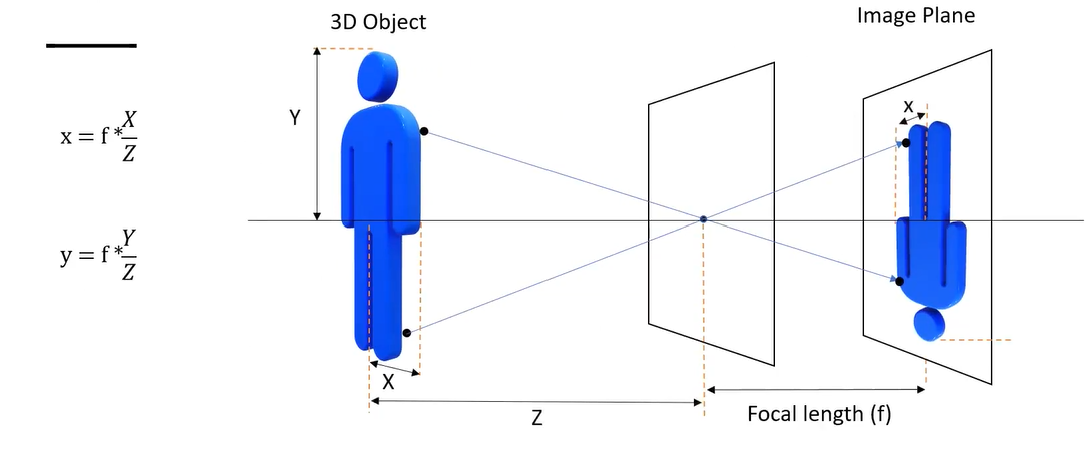
\includegraphics[width = 250pt]{pinholecamera.png}
      \caption{PinHole Camera Example}
      \label{fig: Pinhole Camera}
    \end{figure}

    %

    \subsection{Image Formation}
    Inside of a camera there is a sensor that is a large grid of nodes. These nodes are what eventually become ``pixels'''. Each node on the sensor gets a value between 0 and 255 which represents the digital grayscale image. The value for each node is determined by the strength of the light that hits it. The stronger the light the closer the value is to 255 as 255 is white and 0 is black. Each pixel is essentially an 8 bit representation of the intensity of the light at that position on the sensor.

    \begin{figure}[h!]
      \centering
      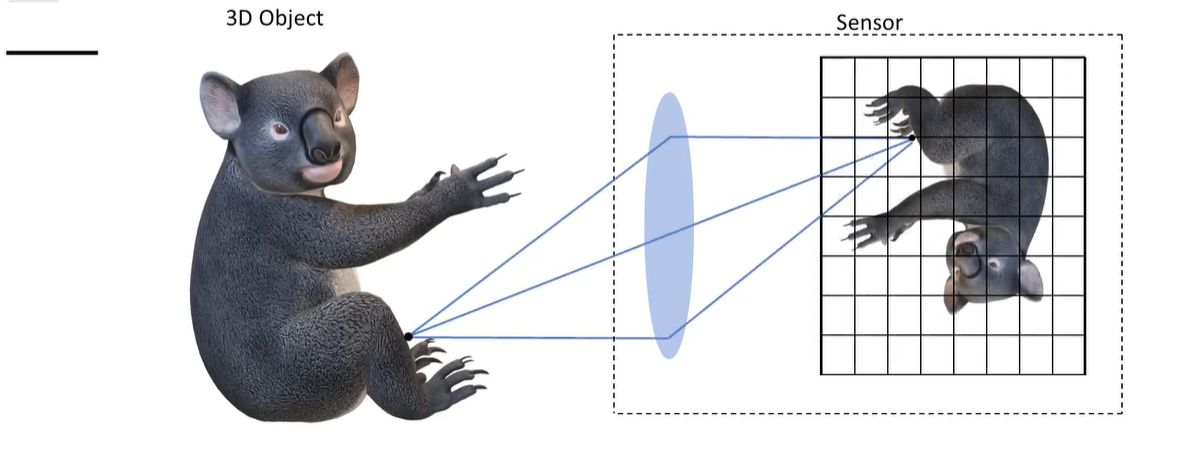
\includegraphics[width=250pt]{koala.png}
      \caption{Greyscale Digitalization }
      \label{fig: Greyscale Representation of an Image}
    \end{figure}



    \newpage
    \clearpage
    \subsection{Bayer Pattern}
    Every pixed only records one color: red, green, or blue. The human eye is much more sensitive to green light than blue or red. The full RGB Image is then formed through a process called demosaicing where 2 two missing values from each pixel are calculated from the neighbouring pixels\\
    \textbf{For example:} If a pixel records the red value, based on the pixels around it the pixel will interpolate what the correct hue for the 2 missing colors.

    \begin{figure}[h!]
      \centering
      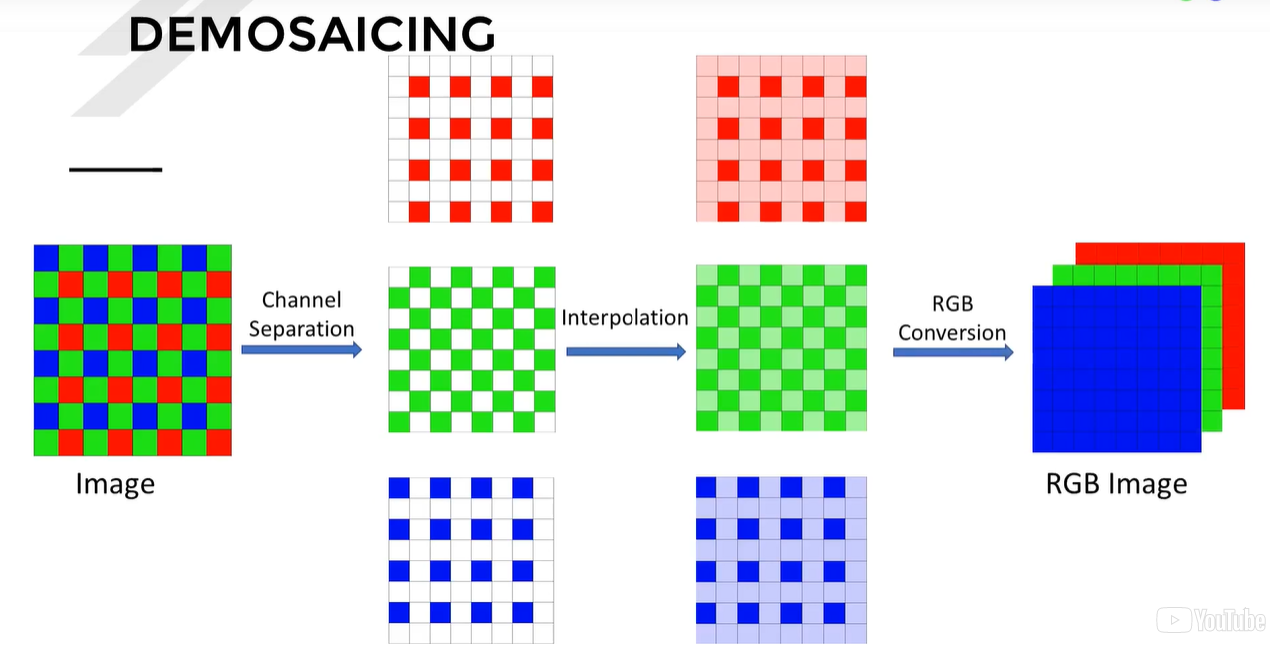
\includegraphics[width=550pt]{demosaicing.png}
      \caption{Process of Demosaicing}
      \label{fig: How the total RGB Image is found through demosaicing}
    \end{figure}

    \subsection{Image Format}
    Once a RGB image is created, they are typically stored and compressed as either Joint Photographic Expert Group (JEPGs) or Portable Network Graphics (PNGs).

    \subsubsection{Image Storage}
    Within a JPEG file the image is broken up into two parts. There is the Image Header and the Data.\\
    \tab - Image Header\\
    \tab\tab - Width\\
    \tab\tab - Height\\
    \tab\tab - No. of channel\\
    \tab\tab - Color Profile\\
    \tab\tab - No. of bits per pixel\\
    The second part is the data which actually contains the RGB values

    \subsection{Image in OpenCV}
    When an image is first read in openCV the image is decompressed and stored in a standardized format. All images are stored into the \textbf{Mat Class} if the C++ version is being used, or a \textbf{Numpy array} if Python is being used.

    \subsubsection{Mat Class}
    The Mat class is similar to a JPEG in structure but the difference is that instead of using RGB values it used BGR. It uses bgr because of historic reasons, aka that is how they initially did it and it makes no sense to back through and change all of the backend code now.

    \newpage
    \clearpage
    \section{Week 1: Reading Images in OpenCV}
    \subsection{Image Formats}
    OpenCV can use two different formats, JPEG and PNG

    \begin{wrapfigure}{r}{400pt}
    \centering
    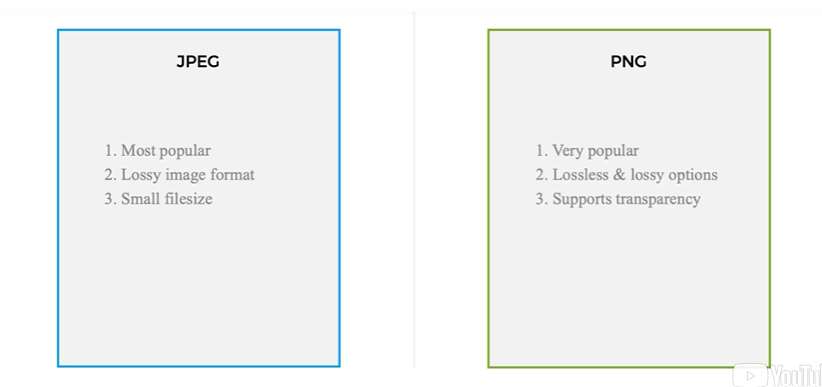
\includegraphics[width=325pt]{jpegvspng.png}
    \caption{\label{fig:jpegvspng}JPEG vs PNG.}
    \end{wrapfigure}


    \subsubsection{JPEG}
    1) Most Popular\\
    2) Loss in image format\\
    3) Small Filesize
    \subsubsection{PNG}
    1) Very Popular\\
    2) Lossless and lossy options\\
    3) Supports transparency\\ \\ \\
    \subsubsection{Transparent Images}

    \begin{wrapfigure}{r}{300pt}
    \centering
    \includegraphics[width=200pt]{Transparentimage.png}
    \caption{\label{fig:Transparentimage}RBG vs Transparent RGB.}
    \end{wrapfigure}
    Contains all three regular channels (Red, Green, Blue) and also contains an `Alpha' channel that acts as a mask (255 or 0). The value that is put into the alpha channel is determined by the Opacity of the pixel. If the pixel is ``Transparent'', then there will be a 0 for that pixel in the Alpha channel. If the pixel is not ``Transparent'', then it will recieve a value of 255.\\
    ***Note: Alpha channels do not neccesarily have to be binary. They can be tertiary or higher if for some reason that kind of masking is wanted/needed. Aka, there can be partial transparencies

    \subsection{Reading The Image (Week One: Getting Started With Images)}
    To load an image through OpenCV use the \textbf{imRread} function. This function is able to handle most, if not all of the image types that you may want to upload (these include JPEG, PNG, etc)

    \subsubsection{Function Syntax: cv2.imread}
    \textbf{$loaded image = cv2.imread(filename, flags)$}\\
    \tab this function (imread) will return the image as a matrix or None if something happened that it was not able to resolve.
    \tab This function has \textbf{two arguments}:\\
    \tab \tab 1) The \textbf{path} of the image file: this can be absolute or relative and is a mandatory argument\\
    \tab \tab 2) \textbf{Flags:} -1, 0, or 1. ***DEFAULT IS ONE***\\
    \indent \indent $cv2.IMREAD\_UNCHANGED$ or -1: Loads an image including the alpha channel (unchanged)\\
    \indent \indent   $cv2.IMREAD\_GRAYSCALE$ or 0: Loads the image in grayscale\\
    \indent \indent  $cv2.IMREAD\_COLOR$ or 1: Loads a color image and throws out transparency\\

    \newpage
    \clearpage
    \subsection{Manipulating Pixels (Week One: Getting Started With Images)}
    \subsubsection{Accessing Values}
    \indent Since the openCV returns things as a matrix of values, you can just access them using the subscript notation of matricies.\\
    IMPORTANT: Numpy saves the matrix in row column format which is the opposite of x,y format. For example if you want to access the pixel to the right of the top left instead of (1,0), which is the cartesian representation of it, it would be [0,1]. This is an important distinction as it will allow you to actually access the correct variables.\\

    \begin{center}
      $print(testImage[0,0])$
    \end{center}


    \subsubsection{Modifying Values}
    Just use a normal python $=$ operation for this. You can either modify a single value or a whole region...that is next\\
    There are a few reasons why people would want to change the values of the pixels. For one, if there is a known issue with the image or a known change that the user might want to change, they need to be able to access and modify the values. For example maybe the edges of the image are blurry so you just set them all to 0 so that there are no false positives.

    \begin{center}
      $testImage[0,0]=200$\\
      $print(testImage)$
    \end{center}

    \subsection{Manipulating Groups of Pixels (Week One: Getting Started With Images)}
    \subsubsection{How To Access A Region}

    \begin{center}
      ROI - Region of Interest\\
      $test\_roi = testImage[0:2,0:4]$\\
    \end{center}

    This code will return a resulting matrix the is 2 rows tall, and 4 columns long. This is a bit counterintuitive because if you count up from 0 (where subscript position starts), and go to the last number then both dimensions are missing 1 element. This is because python is inclusive of the lower bound but non inclusive of the upper bound. \\
    0:2 tells python, hey! Look in this matrix and take out rows 0 and 1, stop before two, and also take columsn 0, 1, 2, 3 and stop before four. Now stich this all together into a matrix and return it! This way the programmer can select a specific part of the iamge that they are interested in using aka, Region of Interest.\\
    To set a region of interest to a specific value all you have to do is take the region, and use the equals operator.

    \begin{center}
      $testImage[0:2,0:4] = 111$
    \end{center}

    \subsection{Displaying An Image}
    Previously learned were the ways that you could display the matrices that made up a specific image and see the values that they contained. Also learned were the ways to modify a pixel or a ROI (Region of Interest). All of this however is pretty much useless as it isn't really possible to visualize a whole picture by just looking at the matricies. There is the need to actually display the image and when using python that is done with Matplotlib.\\
    Matplotlib is a python library for data visualization and does a pretty good job as it. As the name implies, it is a library for plotting math related things. Matplotlib can be installed with a simple, \textbf{pip install matplot lib}. Make sure that you are on the virtualenv that you want to use it for (personally i just install everything system wide I know it is not the right way to do it but it is the way that I do it for ease of use).

    \subsubsection{Function Syntax: plt.imshow() vs cv2.imshow()}
    \indent \textbf{Matplotlib}\\
    \indent \indent - The matplot lib version of the function only has 1 mandatory argument, which is the image in the form of a matrix. A good practice is to also incluse the colorbar() function with it as well as it show a gradient colorbar based on the values.

    \begin{center}
      plt.imshow(matrix)\\
      matrix - Image to be displayed
    \end{center}

    \newpage
    \clearpage

    \textbf{OpenCV}\\
    \indent \indent - The OpenCV version of the function is similar to the Matplotlib version but where it differs is that it opens a separate window to view the image in. This version requires you to have OpenCV installed locally on your computer to run as it uses OpenCV packages.



    \begin{center}
      cv2.imshow(window name, matrix)\\
      \textbf{Read the image:} $boy = cv2.imread(data\_path + ``/images/boy.jpg'')$\\
      \textbf{Display the image using imshow: } $cv2.imshow("Boy", boy)$\\
      \textbf{Wait for user to press a key: } $cv2.waitKey(0)$\\
      \textbf{Destroy the window: } $cv2.destroyAllWindows()$\\
      ***These extra methods will be gone over in the next section***
    \end{center}

    \subsection{Addition Display Utility Functions (OpenCV)}
    \subsubsection{cv2.namedWindow}
    This function creates a display window with a specific name. The name provided is the first argument of the function. The second is a flag that determines whether or not the window can be resized. \\
    The two flags are \textbf{cv2.WINDOW\_NORMAL}, which will all the window to be resized to fit the image that is sent to it, or \textbf{cv2.WINDOW\_AUTSIDZE} which is the default if nothing is sent.
    \subsubsection{cv2.waitKey}
    This function can be used in image and video processing. The only argument that it takes is the milliseconds to wait for a key press. For example if you sent it 100 then it will wait for a key to be pressed for 100ms and proceed if the time has passed or the key has been pressed. If a 0 is passed in then it will wait indefinently until a key is pressed
    \subsubsection{cv2.destroyWindow}
    This function is pretty self explanatory. The only parameter that it takes is the window name. It will then destroy the window
    \subsubsection{cv2.destroyAllWindows}
    Just like destroywindow except it destroys all windows. 






















\end{document}
